\documentclass[border=6pt]{standalone}
\usepackage{tikz}
\usepackage[T1]{fontenc}
\renewcommand{\familydefault}{\sfdefault}
\definecolor{cSor}{HTML}{2B3A67}
\definecolor{cMai}{HTML}{1BAF7A}
\definecolor{cGrey}{HTML}{52514E}
\definecolor{cLine}{HTML}{E4E3DF}
\begin{document}
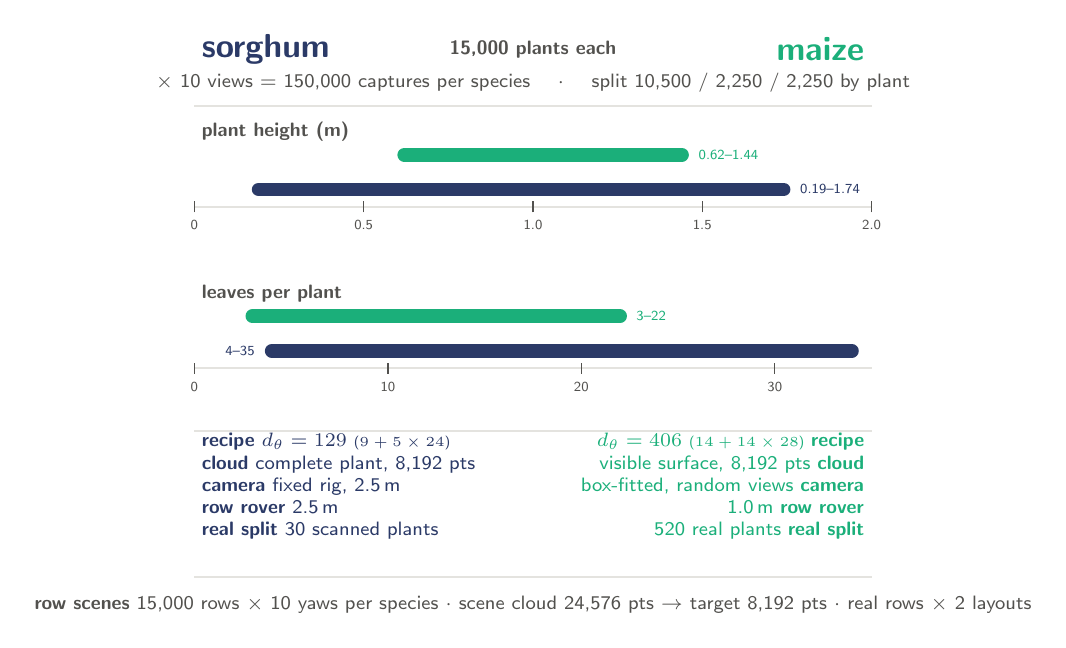
\begin{tikzpicture}[x=1cm,y=1cm]
\scriptsize
\def\W{8.6}
% ---------- header ----------
\node[anchor=west, text=cSor, font=\bfseries\large] at (0,0) {sorghum};
\node[anchor=east, text=cMai, font=\bfseries\large] at (\W,0) {maize};
\node[anchor=center, text=cGrey, font=\bfseries] at (0.5*\W,0) {15{,}000 plants each};
\node[anchor=center, text=cGrey] at (0.5*\W,-0.42) {$\times$ 10 views $=$ 150{,}000 captures per species \quad $\cdot$ \quad split 10{,}500 / 2{,}250 / 2{,}250 by plant};
\draw[cLine, line width=0.6pt] (0,-0.72) -- (\W,-0.72);
% ---------- range bars: height ----------
\node[anchor=west, text=cGrey, font=\bfseries] at (0,-1.05) {plant height (m)};
\begin{scope}[shift={(0,-2.0)}]
  \draw[cLine, line width=0.8pt] (0,0) -- (\W,0);
  \foreach \x/\l in {0/0, 2.15/0.5, 4.3/1.0, 6.45/1.5, 8.6/2.0}
    { \draw[cGrey, line width=0.5pt] (\x,-0.07) -- (\x,0.07); \node[below=1pt, text=cGrey] at (\x,-0.05) {\tiny \l}; }
  % sorghum 0.19-1.74 (stem), maize 0.62-1.44
  \draw[cSor, line width=5pt, line cap=round] (0.817,0.22) -- (7.482,0.22);
  \node[anchor=west, text=cSor] at (7.6,0.22) {\tiny 0.19--1.74};
  \draw[cMai, line width=5pt, line cap=round] (2.666,0.66) -- (6.192,0.66);
  \node[anchor=west, text=cMai] at (6.31,0.66) {\tiny 0.62--1.44};
\end{scope}
% ---------- range bars: leaves ----------
\node[anchor=west, text=cGrey, font=\bfseries] at (0,-3.1) {leaves per plant};
\begin{scope}[shift={(0,-4.05)}]
  \draw[cLine, line width=0.8pt] (0,0) -- (\W,0);
  \foreach \x/\l in {0/0, 2.457/10, 4.914/20, 7.371/30}
    { \draw[cGrey, line width=0.5pt] (\x,-0.07) -- (\x,0.07); \node[below=1pt, text=cGrey] at (\x,-0.05) {\tiny \l}; }
  \draw[cSor, line width=5pt, line cap=round] (0.983,0.22) -- (8.35,0.22);
  \node[anchor=east, text=cSor] at (0.86,0.22) {\tiny 4--35};
  \draw[cMai, line width=5pt, line cap=round] (0.737,0.66) -- (5.406,0.66);
  \node[anchor=west, text=cMai] at (5.52,0.66) {\tiny 3--22};
\end{scope}
\draw[cLine, line width=0.6pt] (0,-4.85) -- (\W,-4.85);
% ---------- per-species facts ----------
\node[anchor=west, align=left, text=cSor] at (0,-5.55) {%
  \textbf{recipe} $d_\theta = 129$ {\tiny($9 + 5 \times 24$)}\\
  \textbf{cloud} complete plant, 8{,}192 pts\\
  \textbf{camera} fixed rig, 2.5\,m\\
  \textbf{row rover} 2.5\,m\\
  \textbf{real split} 30 scanned plants};
\node[anchor=east, align=right, text=cMai] at (\W,-5.55) {%
  $d_\theta = 406$ {\tiny($14 + 14 \times 28$)} \textbf{recipe}\\
  visible surface, 8{,}192 pts \textbf{cloud}\\
  box-fitted, random views \textbf{camera}\\
  1.0\,m \textbf{row rover}\\
  520 real plants \textbf{real split}};
\draw[cLine, line width=0.6pt] (0,-6.7) -- (\W,-6.7);
% ---------- rows footer ----------
\node[anchor=center, text=cGrey] at (0.5*\W,-7.05) {\textbf{row scenes} 15{,}000 rows $\times$ 10 yaws per species $\cdot$ scene cloud 24{,}576 pts $\to$ target 8{,}192 pts $\cdot$ real rows $\times$ 2 layouts};
\end{tikzpicture}
\end{document}
